\section{Charging Station Design}

The design of the charging station is displayed in \autoref{fig:class-diagram}. Central to the system is the \textit{stationControl} class, which handles all interaction with the user, through various interfaces (display, door and rfid detector). It also interacts with the \textit{chargeController} through another interface. The \textit{chargeController} meanwhile interfaces with the USB charger, cobntrolling it, and also displays charging status on the display through the display interface. 

\begin{figure}[h]
  \centering
  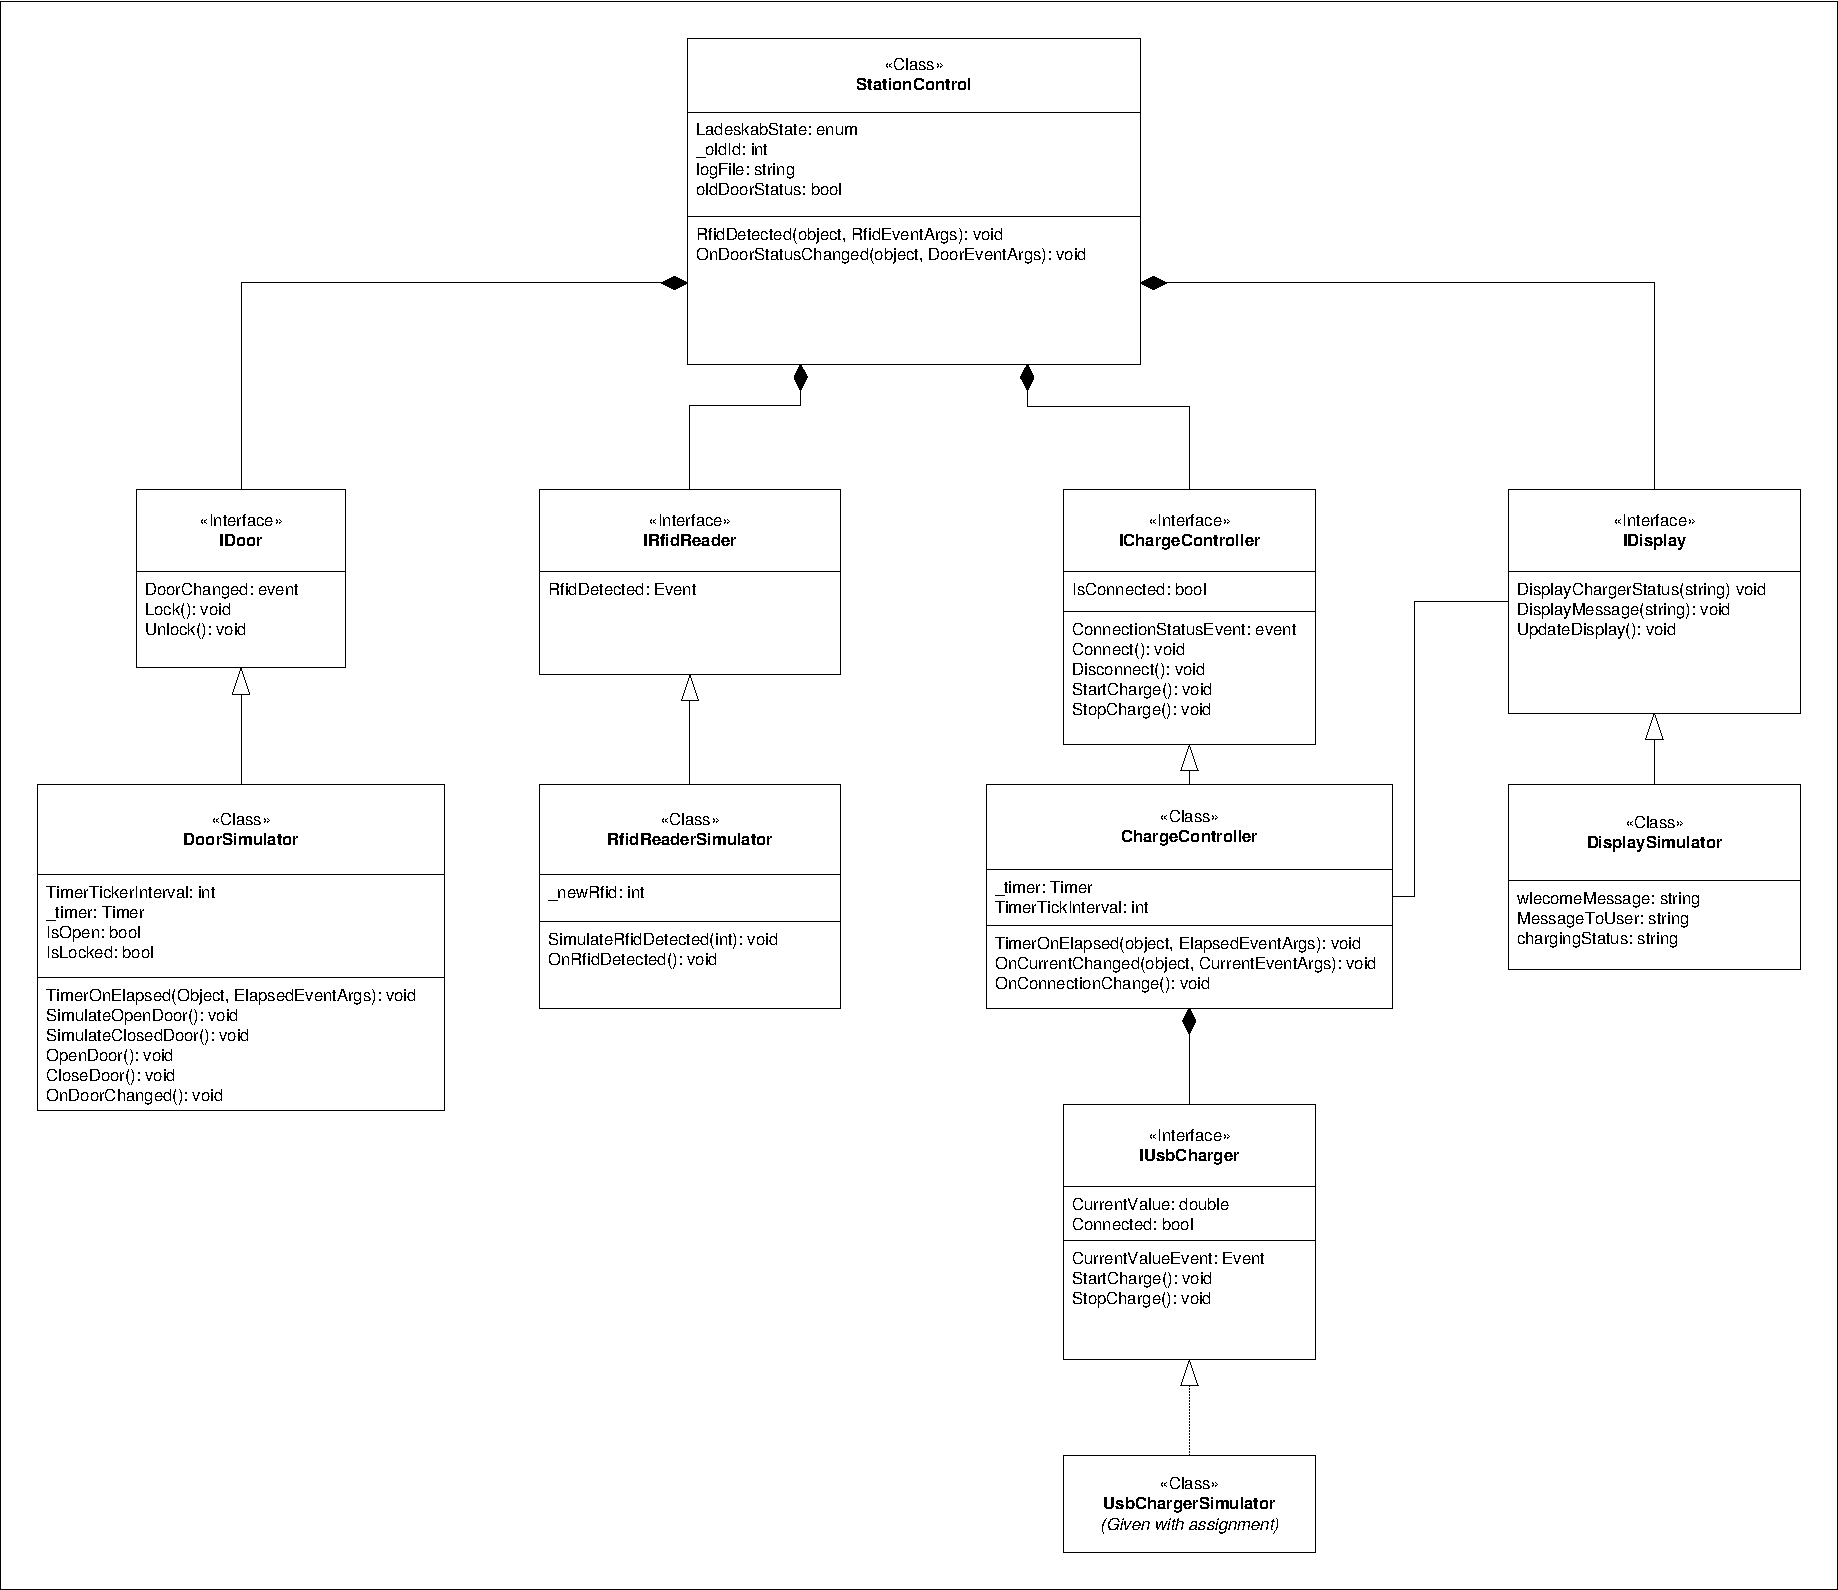
\includegraphics[width=\textwidth]{02-Body/images/ChargingStation_classDiagram.pdf}
  \caption{Class diagram for the charging station system}
  \label{fig:class-diagram}
\end{figure}

The charging station is first activated by the door opening, causing the station to ask the user to connect the phone. The user then connects the phone and closes the door, which causes the station to ask for an rfid. If the phone has not been correctly connected (as cheked by the chargeController) the station reports this to the user through the display. 